\subsection{Windows Azure Storage}
Windows Azure Storage \cite{DBLP:conf/sosp/CalderWONSMXSWSHUKEBMAAHHBDAMSMR11}, WAS for short, is a system developed by Microsoft for the Azure cloud platform and it is in production since 2008.
Unlike a classic distributed file-system where the only primitive offered is the file, WAS offers three different primitives to clients:
\begin{itemize}
    \item a blob storage to process unstructured data,
    \item a table storage to process structured data in tuples, and
    \item a queue system to build message-passing based systems.
\end{itemize}
Typically data flowing into and out of the system is saved in blob storage, sent to workers as queue items and processed using the table store.

WAS was designed around a global namespace which allows clients to access data in any deployment in the world using the same addressing scheme.
Data in the system can be accessed with a url built from three components: \emph{account~name}, \emph{partition~name} and \emph{object~name}, which can uniquely identify all objects available in the system worldwide.
While account name is used to identify the client, identification of the data objects varies according to the type of object: blobs are uniquely identified by partition~name, tuples in table storage are identified by a composite primary key (partition~name, object~name) and for queues, the partition~name identifies the queue and the object~name the specific message within that queue.

\subsubsection{Architecture}
\begin{figure}[h]
\caption{Windows Azure Storage architecture diagram}
\label{fig:was-architecture}
\centering
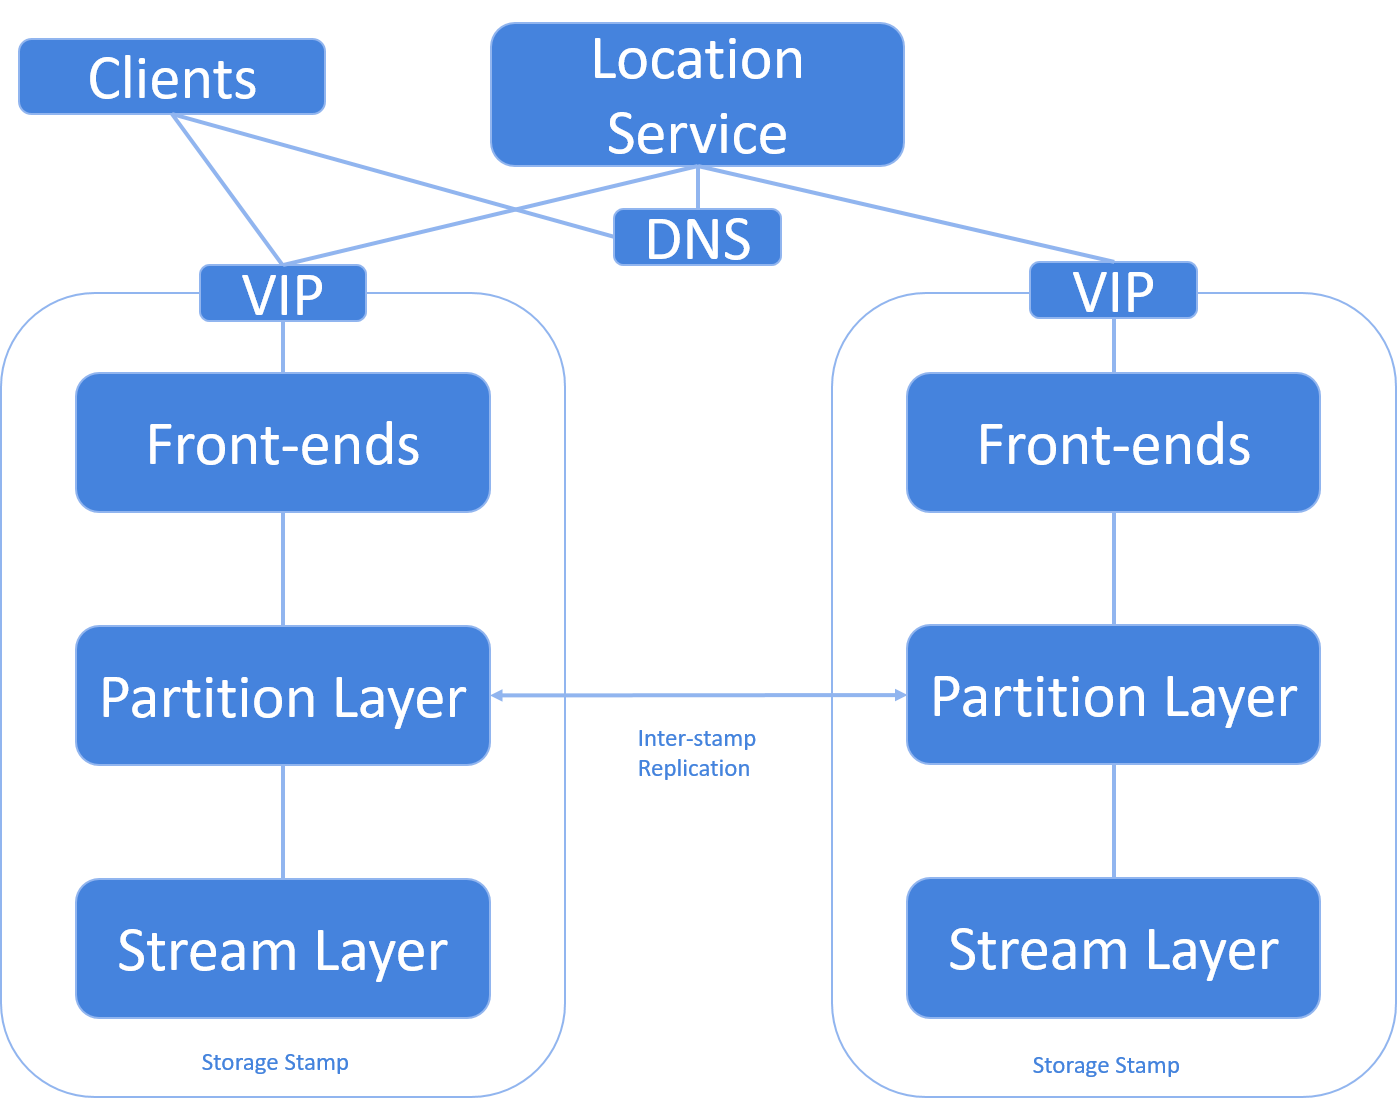
\includegraphics[width=1.0\textwidth]{images/windows-azure-storage.png}
\end{figure}

The architecture of the system, shown in Figure \ref{fig:was-architecture}, includes two separate systems:
\begin{inparaenum}[i)]
    \item the location service (LS) and
    \item the storage stamps (SS).
\end{inparaenum}
The location service handles the global namespace and as such, the lifecycle of accounts and the management of storage stamps.
This involves managing the association of accounts to storage stamps, and coordination of the replication of account data between stamps for disaster recovery purposes (async replication).
The location service is itself distributed on two geographical zones for redundancy and fault tolerance.

Storage stamps, on the other hand, perform the physical storage of data and respond to all user queries.
Each storage stamp is a cluster of racks, where each rack is a separate failure domain with redundant connectivity and power supply, and can store up to 30 petabytes (at the time the paper was published).
The target utilization for a storage stamp is 70\% and if it raises accounts are migrated to other stamps.
Each storage stamp is divided into three layers which perform different functions:
\begin{itemize}
    \item the \emph{Stream Layer} stores data on disk, its design is very close to that of other distributed file-systems,
    \item the \emph{Partition Layer} implements the higher level data abstractions discussed, provides transactions and strong consistency for objects, caches data and uses the Stream Layer to store the data for the objects, and finally,
    \item the \emph{Front End Layer}, a stateless component that performs routing of requests to the appropriate Partition Layer process and streams large objects directly from the Stream Layer as an optimization for large files.
\end{itemize}

\paragraph{The Stream Layer}

The \emph{Stream Layer} implements the basic storage primitives for the system and it is accessed by the Partition Layer (the client).
Its design is that of a append-only filesystem, and the interface provided to clients offers the usual operations:
\begin{inparaenum}[i)]
    \item open,
    \item close,
    \item delete,
    \item rename,
    \item read,
    \item append, and
    \item concatenate.
\end{inparaenum}
Operations in the stream layer work on streams, large files built as a list of pointers to extents.
Extents are physical file stored on the NTFS filesystem that contain the data, as a list of blocks.

\emph{Blocks} are small data units (up to 4MB) with a check-sum and they are the minimum unit the system operates on.
Reads and writes operate on whole blocks and when written, the blocks are atomically appended to an extent.
Writes also support appending multiple blocks as an atomic operation, a ``multi-block'' write.
Reading less than one block is also not supported, as read operations verify the chechsums for block themselves (and the checksum cannot be verified by reading only a part of the block).
If less than a block is requested by clients an entire block is loaded into memory and the extra data is simply discarded.

\emph{Extents} are just a list of appended blocks that can grow up to 1GB in size.
Extents, much like blocks in HDFS, are the unit of replication in the stream layer and, unless there are errors, there are three copies of each available in the system.
Unless an extent is last in a particular stream, it is sealed.
A sealed extent can no longer be appended to and is completely immutable.
Sealed blocks can also be erasure coded, depending on policy.
Erasure coding in WAS is described in detail in a separate paper \cite{DBLP:conf/usenix/HuangSXOCG0Y12}.
To avoid excessive fragmentation of small objects, the stream layer appends multiple objects to the same block or the same extent, depending on the size.

\emph{Streams} are the file-like primitive provided to clients by the stream layer.
Every stream has a name in the name-space of the stamp (which is maintained at the stream layer), and it is a list of pointers to extents.
Representing streams as list of pointers enables a very efficient concatenation operation, where two or more streams can be merged by just concatenating the list of pointers but without modifying the existing extents.
All of the extents in a stream but the last are sealed.

The stream layer is organized as two different components:
\begin{itemize}
    \item the Stream Manager (SM), a component similar to HDFS's namenode and
    \item the Extent Nodes (EN), components that perform a function similar to that of HDFS datanodes.
\end{itemize}

The \emph{Stream Manager} is a group of nodes, coordinating using Paxos, that performs functions equivalent to those of a HDFS namenode.
Such functions include assigning extents, both primary and replicas, to extent nodes, performing periodic polling and re-replication of under-replicated blocks and the storage of metadata on streams.
Streams are managed solely by the Stream Manager as a set of pointers to extents stored by Extent Nodes.

\emph{Extent Nodes}, on the other hand, manage the physical storage of extents on disk.
Each node completely manages a set of disks where extents are saved as NTFS files.
For each extent the nodes also store an index that identifies block boundaries within the stream.
Extent nodes also perform synchronous replication of extents to other nodes both during client writes and during re-replication as scheduled by the Stream Manager.

\paragraph{The Partition Layer}

The \emph{Partition Layer} builds upon the storage primitives of the Stream Layer to provide higher level APIs to application developers.
Clients that access Windows Azure Storage can only use operations provided by the Partition Layer and cannot access the Stream Layer directly.
The APIs provided to external clients allow users to store data and manipulate it in three different types of objects:
\begin{inparaenum}[i)]
    \item blobs,
    \item tables and
    \item queues.
\end{inparaenum}
Additionally, the Partition Layer provides transactional behaviour for all supported data models, load-balancing and object namespacing within the stamp and finally, inter-stamp replication for disaster recovery and balancing purposes.
The inter-stamp replication works by asynchronously replicating all data for an account from a primary stamp, where all the queries are routed by the LS, to a secondary stamp in a different geographic region.
The secondary stamp can be promoted to primary both if the primary fails (disaster recovery) or if its load raises above a set threshold (load balancing).

All internal state for the Partition Layer is stored and processed in Object Tables (OT), an internal abstraction providing SQL-like tables that can grow to several petabytes.
All user-facing abstractions, as well as internal functions are stored in such tables, which are in turn persisted by the Stream Layer.
The Partition Layer manages OTs by dividing them in ranges and assigning ranges to nodes.
The Partition Layer is itself organized as a set of three different components:
\begin{itemize}
    \item a Partition Manager (PM) that splits the object table and assigns it to Partition Servers. It manages failures of Partition Servers and does load balancing by re-assigning partitions to other servers,
    \item Partition Servers (PS) which serve requests for the partition of OTs they are managing, and
    \item a Lock Service (LS) which provides a Paxos \cite{DBLP:journals/tocs/Lamport98} lock service used to elect a Partition Manager from the set of Partition Servers and to detect failures in Partition Servers.
\end{itemize}